This lab expanded on the concepts of asymmetric encryption through the use of\newline
GPG/GnuPG (GNU Privacy Guard) to produce, sign and verify public and private keys.

\section{Creating test users}\label{sec:testUsers}
For this lab, two test users were created and used to execute the necessary commands.

\subsection{Elevating the terminal}\label{subsec:sudo}
To add users to the system, administrative privileges are required.
To gain the necessary privileges, the command "sudo -s" or "sudo bash" can be entered
(both commands are functionally identical) which will change the terminal to be at root level.

\begin{figure}[H]
    \centering
    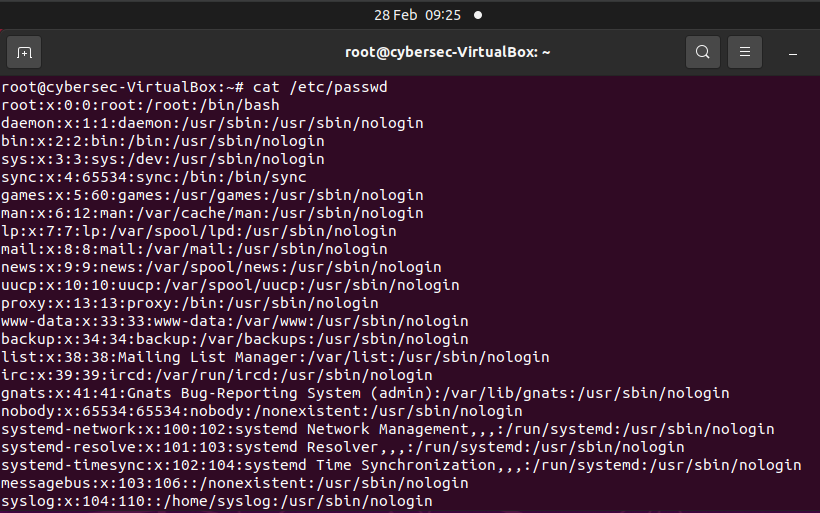
\includegraphics[width=.9\linewidth]{lab2/1}
    \caption{Elevating the terminal.}
    \label{fig:sudo}
\end{figure}

\subsection{Creating Bob and Alice}\label{subsec:createUsers}
With the elevated privileges gained from being a superuser, it is now possible to add users to the system using
"adduser" followed by the given username.
A password will then be necessary, followed by optional information such as phone numbers, which are left empty
for this lab.

\begin{figure}[H]
    \centering
    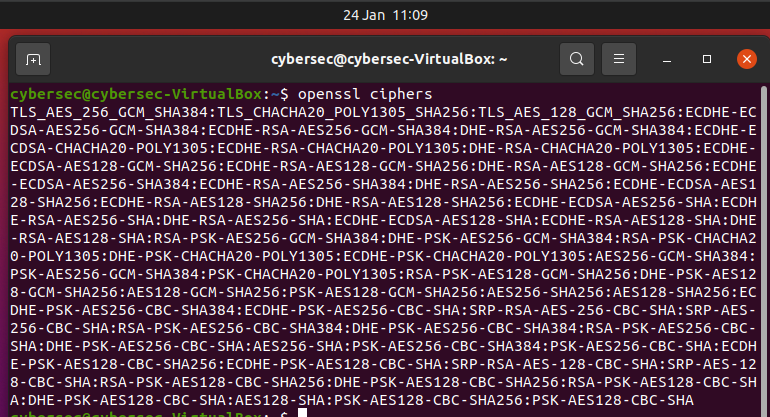
\includegraphics[width=.6\linewidth]{lab2/3}
    \caption{Creating user 'bob'}
    \label{fig:createBob}
\end{figure}

\begin{figure}[H]
    \centering
    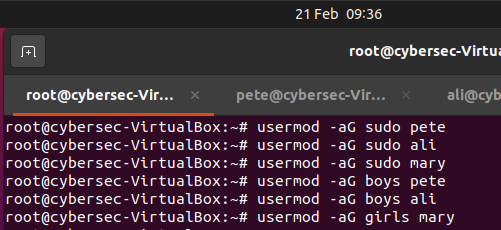
\includegraphics[width=.6\linewidth]{lab2/2}
    \caption{Creating user 'alice'.}
    \label{fig:createAlice}
\end{figure}

For ease of access, multiple terminal tabs can be open at a time, so I elected to use one for the superuser root,
and one each for Bob and Alice.

\begin{figure}[H]
    \centering
    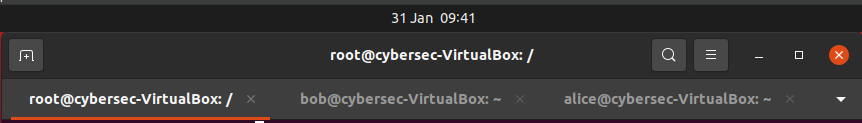
\includegraphics[width=.9\linewidth]{lab2/4}
    \caption{Multiple terminal tabs.}
    \label{fig:terminalTabs}
\end{figure}

I also added these new users to the "sudo" group, allowing them to also use the sudo command to execute commands
with elevated permissions.

\begin{figure}[H]
    \centering
    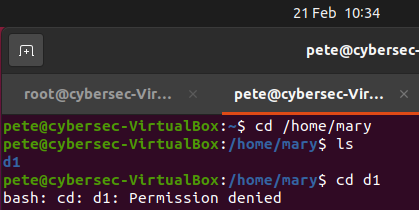
\includegraphics[width=.8\linewidth]{lab2/5}
    \caption{Adding bob and alice to sudo.}
    \label{fig:sudoAdd1}
\end{figure}

\begin{figure}[H]
    \centering
    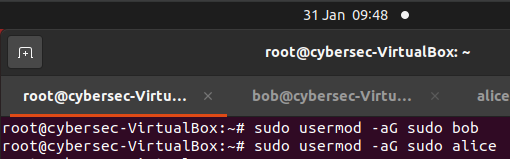
\includegraphics[width=.8\linewidth]{lab2/5b}
    \caption{Adding bob and alice to sudo.}
    \label{fig:sudoAdd2}
\end{figure}

It is possible to switch the active terminal user using the command "su" followed by the account to switch to,
and then the password of the given account.

\begin{figure}[H]
    \centering
    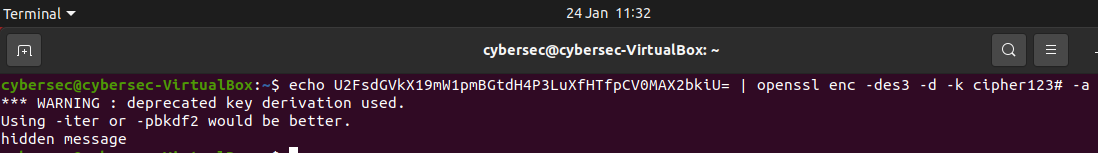
\includegraphics[width=.9\linewidth]{lab2/5c}
    \caption{Switching the active terminal user. Note the prompt about running commands as an administrator,
    which signifies that they were successfully added to the sudo group.}
    \label{fig:suBobAlice}
\end{figure}

\pagebreak

\section{Exchanging files over an insecure channel}\label{sec:tmpExchange}
On standard Linux distributions, the /tmp directory is a public directory accessible to all users.
For this reason, it is therefore unsecure, as every user on the system can access the files placed there.


